\documentclass[letterpaper, 12pt]{article}
\usepackage[top=2 cm, bottom=2 cm,left=1.5 cm, right=1.5 cm]{geometry}

\usepackage[spanish,es-nodecimaldot]{babel}
\usepackage[utf8]{inputenc}
\usepackage{csquotes}

\setlength{\parindent}{1cm}
\pagestyle{empty}

\usepackage[colorlinks=true, urlcolor=blue, linkcolor=red]{hyperref} % Para insertar hipervínculos
\usepackage{amsmath}
\usepackage[outputdir=aux]{minted}
\usepackage{amssymb}
\usepackage{multicol}
\usepackage{enumerate}
\usepackage{graphicx} % Incluir imágenes
\usepackage[document]{ragged2e}
\usepackage{mathrsfs}
\usepackage[T1]{fontenc}
\usepackage[table,xcdraw]{xcolor}
\usepackage{float} %required for the placement specifier H
\makeatletter
\makeatother
% -----------------------------------------------

% Preámbulo

\title{Tarea 2: }
\author{Christopher Gómez}
\date{Marzo 2022}

\begin{document}
\parbox[t]{.5\linewidth}{
    \centering
    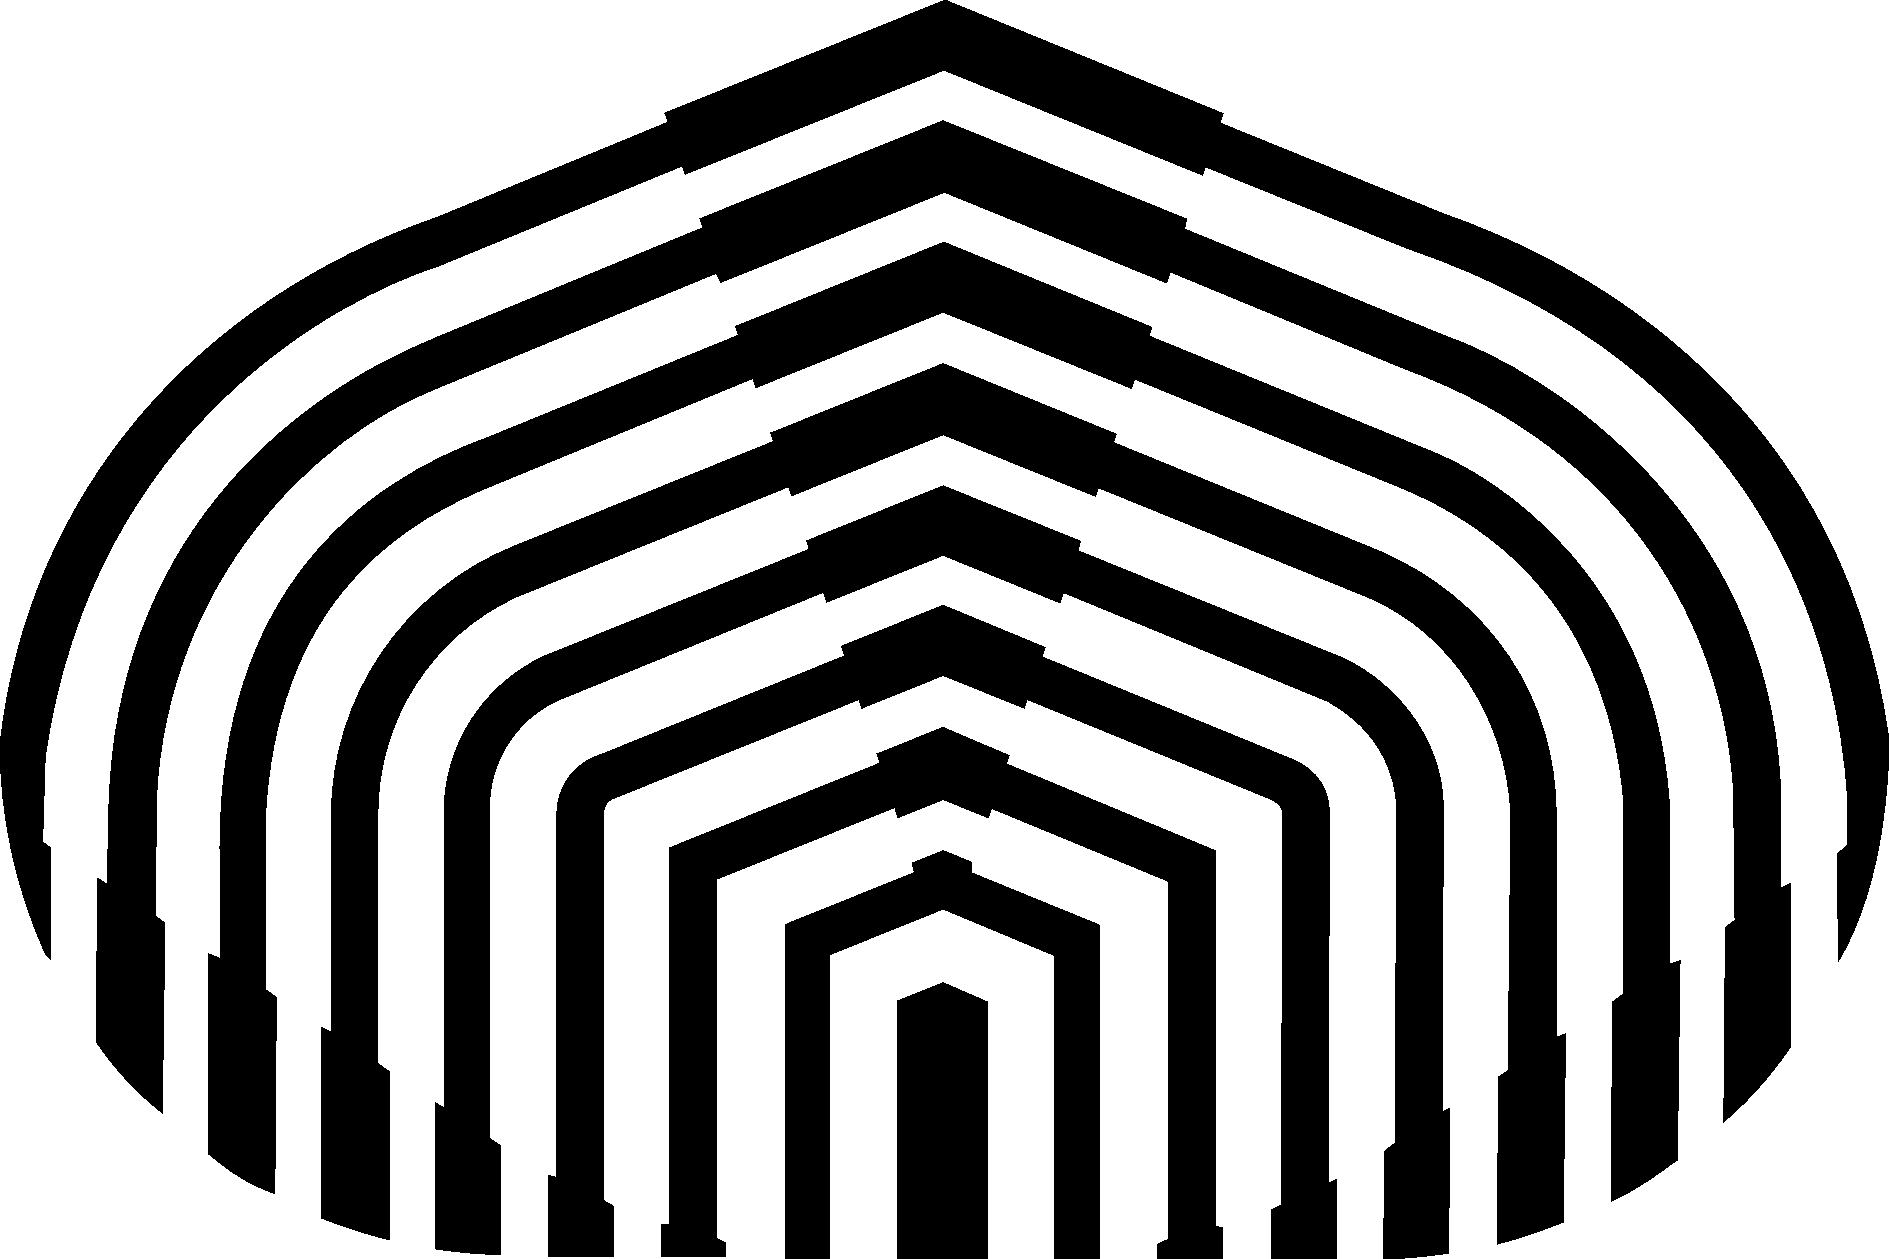
\includegraphics[scale=0.4]{logo.png}
    \begin{center}
        UNIVERSIDAD SIMÓN BOLÍVAR \\
        CI-5651 - Diseño de Algoritmos I \\
        Prof. Ricardo Monascal \\
    \end{center}
}
\hfill \framebox[5.5cm][c]{
        \parbox[t]{.8\linewidth}{
        \centering
       Resuelto por:\\ Christopher Gómez
        }}

\phantom{This text will be invisible} \\
\centerline {\textbf{Tarea 2: }}
\justify

\begin{enumerate}

% -------- PREGUNTA 1 --------

\item  En un nuevo túnel, diversos productos quieren colocar vallas para promover sus productos. Usted debe dar los permisos apropiados para colocar estas vallas y no desea que ninguna de estas se intersecte con otra (sin embargo, dos vallas pueden estar una al lado de la otra, esto es, compartir un extremo).

Las propuestas de publicidad incluyen el punto en donde la valla empezará (en metros, contando desde el inicio del túnel) y el tamaño de la misma (también en metros). Ninguna de estas condiciones es negociable. Los departamentos de publicidad de cada uno de los productos interesados han llegado a la conclusión de que quieren la valla en ese exacto punto, con esas exactas dimensiones o prefieren no colocar publicidad alguna. Todas las vallas se colocarán planas en una sola pared del túnel.

Dadas $n$ peticiones de publicidad, donde la $i$-ésima petición tiene $p_i$ (el punto de inicio de la valla) y $t_i$ (el tamaño de la valla), diseñe un algoritmo \emph{eficiente} que permite escoger un conjunto maximal de peticiones tal que ninguna valla intersecte con otra.

Su algoritmo debe usar tiempo $O(n\log n)$ y memoria adicional $O(n)$.

Justifique \emph{informalmente} por qué su algoritmos es correcto y cumple con el orden asintótico propuesto. \\

Este problema puede ser resuelto utilizando un algoritmo voraz, el cual consiste en ordenar las peticiones de publicidad en orden creciente de sus puntos finales $(p_i + t_i)$ y luego recorrer la lista, seleccionando la que se está considerando si no se superpone con las ya seleccionadas. Veámoslo en pseudocódigo:

\begin{minted}{python}
    def publicidad(peticiones: Conjunto[Peticion]) -> Conjunto[Peticion]:
        peticiones.odernar(lambda p: p.comienzo + p.tamaño)
        seleccionadas = {}
        for peticion in peticiones:
            if not se_superpone(peticion, seleccionadas):
                seleccionadas.añadir(peticion)
        return seleccionadas
\end{minted}

Una noción intuitiva de por qué este algoritmo es correcto es que, al seleccionar la petición con el punto final más pequeño que no se superpone con las ya seleccionadas, se deja el mayor espacio posible para las peticiones restantes. Esto es, se selecciona la petición que deja el mayor espacio a la derecha para las peticiones restantes.

Agregando un poco más de formalidad, definamos que un conjunto de peticiones es prometedor si constituye un subconjunto de alguno de los conjuntos maximales de peticiones que no se superponen. Luego, el algoritmo voraz es correcto si en cada iteración del ciclo, el conjunto de peticiones seleccionadas es prometedor, hasta que no hay más peticiones por considerar.

\textbf{Caso base:} El conjunto vacío es prometedor, ya que es subconjunto de cualquier conjunto. En particular, de los conjuntos solución.

\textbf{Caso inductivo:} Supongamos que P es prometedor. En una iteración dada se selecciona una petición $p$ tal que:

\begin{enumerate}
    \item No se superpone con ninguna de las peticiones seleccionadas.
    \item Tiene el punto final más pequeño de las no seleccionadas.
\end{enumerate}

Se tiene entonces que $P \cup \{p\}$ es prometedor, ya que de no serlo (un subconjunto maximal de peticiones que no se superponen), entonces existen al menos dos peticiones $q_1$ y $q_2$ no seleccionadas que no se superponen entre sí, ni con ninguna de las peticiones seleccionadas, y que tienen puntos finales más pequeños que $p$ capaces de sustituir a $p$ para formar un conjunto más grande. Pero esto es una contradicción, ya que $p$ fue seleccionada por tener el punto final más pequeño de las no seleccionadas.

Por lo tanto, el invariante se mantiene en todo momento y que el algoritmo es correcto.

Luego, el algoritmo tiene un tiempo de ejecución de $O(n \log n)$ debido a la ordenación inicial, que se puede implementar en $O(n \log n)$, y el recorrido por la lista de peticiones ordenadas una sola vez, que tarda $O(n)$, ya que se puede implementar \texttt{se\_superpone} en $O(1)$, manteniendo una variable que almacene el último punto final seleccionado y comparando con este en cada iteración.

Además, utiliza memoria adicional $O(n)$ para almacenar las peticiones, y una implementación \emph{in-place} de la ordenación no requiere más que memoria adicional $O(1)$, por lo que cumple con el orden asintótico propuesto.

Una implementación de este algoritmo en Rust se puede encontrar \href{https://gitfront.io/r/chrischriscris/swaWSXShzVoW/Tareas-CI5651-EM2024/tree/tarea2/ej1/}{aquí}. \\

% -------- PREGUNTA 2 --------


\item Considere las siguientes definiciones:

\textbf{Conjuntos definitivos de firmas funcionales}

Considere un conjunto de tipos $T$ y sea $F$ todas las firmas de funciones posibles entre los tipos de $T$ .

Por ejemplo, si $T = \{A, B, C\}$ entonces $F$ contiene

\begin{multicols}{3}
\begin{itemize}
    \item $A \rightarrow A$
    \item $A \rightarrow B$
    \item $A \rightarrow C$
    \item $B \rightarrow A$
    \item $B \rightarrow B$
    \item $B \rightarrow C$
    \item $C \rightarrow A$
    \item $C \rightarrow B$
    \item $C \rightarrow C$
\end{itemize}
\end{multicols}

Diremos que un subconjunto $F' \subseteq F$ es \emph{definitivo} si cada tipo ocurrente en $F'$ aparece a lo sumo una vez como imagen en $F'$.

Por ejemplo, para el mismo $T$ anterior:

\begin{itemize}
    \item $\{A \rightarrow B, B \rightarrow C\}$ es definitivo
    \item $\{A \rightarrow B, C \rightarrow B\}$ no es definitivo.
\end{itemize}

\textbf{Matroide asociada}

Dado un conjunto de tipos $T$ y su conjunto de todas las firmas de funciones $F$, definimos $M_T = (F, I)$, donde $F' \in I$ si y sólo si $F'$ es definitivo. \\

\textbf{Potencial de una firma funcional}

Definimos el \emph{potencial} de una firma de función $X \rightarrow Y$ como la cantidad de funciones posibles que existen con $X$ como dominio y $Y$ como imagen. Recordemos que esto es igual a $|Y|^{|X|}$. Puede suponer que todos los tipos tienen al menos un elemento ($T$ no contiene al tipo vacío).

El potencial de un conjunto de firmas de funciones es la suma del potencial para cada una de la firmas que contiene.

Se desea que:

a) Demuestre que $M_T$ es una matroide.
b) Plantee una función de costo $w$ de tal forma que para la matroide pesada $M_T$ , con $w$ como función de peso, los sub-conjuntos óptimos son los subconjuntos \emph{definitivos} con \emph{potencial máximo}.

\end{enumerate} \vspace{4mm}

\end{document}
